The stock price movements have similarities with electricity prices in terms of its non-linearity and chaotic/dynamic nature. Investors must take into account these factors when handling time series that are non-stationary, noisy and have structural breaks. In addition macro-economical elements significantly influence stock and electricity prices, e.g the economy in general, politics, bank rates and expectations of investors could be examples of such influences. In \cite{stockForecasting} they presented an Artificial Neural Network (ANN) approach to forecasting stock prices. These networks are powerful tools when solving complex problems because they possess qualities such as learning, generalizing, parallel processing and error endurance. The ANN in In \cite{stockForecasting} is based on a Wavelet De-Noising-based Back Propagation (WDBP) which has the ability to filter away undesirable characteristics from the input. The purpose of the filtering is to separate stock price characteristics away from noise so that prediction will have better chances of accuracy when all undesirable has been discarded. The prediction is then used by investors in their attempt to gain profits. 

A day-ahead forecasting algorithm that predicts electricity prices in the market based on Artificial Neural Network (ANN) and Similar Days Method (SDM) is described in \cite{pjmForecast}. The purpose is to give close estimates for several days to come. The estimates can be used by electricity traders in their decision making but also by transmission companies for different purposes. The companies can use it for scheduling a short-term generator outage in order to predict where it is most inexpensive. It can also be used by actual producers of energy to strategically bid into the market to increase prices. The price estimate itself plays a huge role in decision making in all of these examples.

The combination of ANN and SDM is an attempt to simplify the ANN and make the prediction more accurate. The SDM technique averages five days that are similar to the corresponding forecast day. This makes the algorithm consider the influence of the most similar days and their price development compared to the day we wish to forecast. An actual forecast can be seen in figure ~\ref{fig:actualForecastMay13}.
\begin{figure}[h!]
\centering
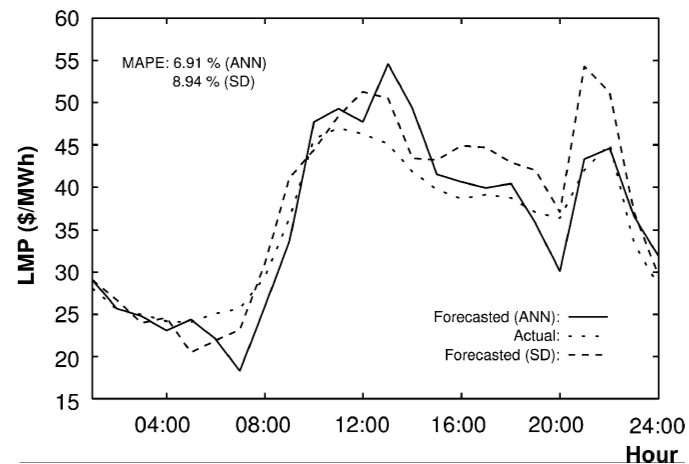
\includegraphics[width=0.8\linewidth,natwidth=898,natheight=587]{billeder/SDMANNAccuracy.png}
\caption{Actual day-ahead forecast from Saturday, May 13, 2006 \cite{pjmForecast}}
\label{fig:actualForecastMay13}
\end{figure}
The ANN is trained with only 45 days from the day before the forecast and 45 days before and after the forecast day in the previous year.
\\[0.5cm]
Prediction algorithms are not only used by electricity traders but can also be a part of various applications. In \cite{22} they introduce an intelligent electricity broker (IEB) that is integrated into Smart Grids where it; 1) provides provision of en energy storage; 2) attempts to lower the electricity bill, and 3) optimally utilizes electricity during peak and low-peak energy production periods. The prediction algorithm is used by a decision algorithm to locate points in time where it is most feasible for the owner of the smart grid to either sell stored energy or buy energy if storage is low. It helps the system to lower the total amount of energy costs to the owner and also utilize the energy in the most intelligent way.
 